\begin{center}
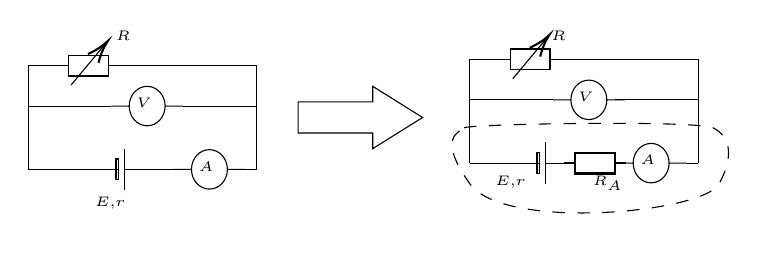
\begin{tikzpicture}[x=0.75pt,y=0.75pt,yscale=-1,xscale=1]
%uncomment if require: \path (0,300); %set diagram left start at 0, and has height of 300

%Straight Lines [id:da9223803374157449] 
\draw    (200,160) -- (230,160) ;
%Straight Lines [id:da4800046187933087] 
\draw    (310,129.5) -- (280,129.5) ;
%Shape: Battery [id:dp11572428456821915] 
\draw   (230,160) -- (243.5,160) (246.5,150) -- (246.5,170) (246.5,160) -- (260,160) (242.3,155) -- (243.5,155) -- (243.5,165) -- (242.3,165) -- (242.3,155) -- cycle ;
%Straight Lines [id:da5053925872800769] 
\draw    (200,110) -- (200,160) ;
%Straight Lines [id:da4775642533714568] 
\draw    (304.6,160) -- (310,160) ;
%Straight Lines [id:da025516599512321214] 
\draw    (310,110) -- (310,160) ;
%Shape: Output [id:dp20535874065942084] 
\draw   (278.65,160) .. controls (278.65,154.75) and (282.52,150.5) .. (287.3,150.5) .. controls (292.08,150.5) and (295.95,154.75) .. (295.95,160) .. controls (295.95,165.25) and (292.08,169.5) .. (287.3,169.5) .. controls (282.52,169.5) and (278.65,165.25) .. (278.65,160) -- cycle (270,160) -- (278.65,160) (304.6,160) -- (295.95,160) ;
%Straight Lines [id:da8691520573396538] 
\draw    (260,160) -- (270,160) ;
%Straight Lines [id:da22747916883790165] 
\draw    (200,110) -- (214,110) ;
%Shape: Resistor [id:dp2800596618552471] 
\draw   (219.4,115) -- (238.6,115) -- (238.6,105) -- (219.4,105) -- (219.4,115) -- cycle (214,110) -- (219.4,110) (238.6,110) -- (244,110) ;
%Straight Lines [id:da15708168083551777] 
\draw    (220.67,119.33) -- (237.04,99.7) ;
\draw [shift={(238.33,98.16)}, rotate = 129.83] [color={rgb, 255:red, 0; green, 0; blue, 0 }  ][line width=0.75]    (10.93,-3.29) .. controls (6.95,-1.4) and (3.31,-0.3) .. (0,0) .. controls (3.31,0.3) and (6.95,1.4) .. (10.93,3.29)   ;

%Straight Lines [id:da11312699458388331] 
\draw    (244,110) -- (310,110) ;
%Straight Lines [id:da6739961140053903] 
\draw    (274.6,129.5) -- (280,129.5) ;
%Shape: Output [id:dp7899198086186321] 
\draw   (248.65,129.5) .. controls (248.65,124.25) and (252.52,120) .. (257.3,120) .. controls (262.08,120) and (265.95,124.25) .. (265.95,129.5) .. controls (265.95,134.75) and (262.08,139) .. (257.3,139) .. controls (252.52,139) and (248.65,134.75) .. (248.65,129.5) -- cycle (240,129.5) -- (248.65,129.5) (274.6,129.5) -- (265.95,129.5) ;
%Straight Lines [id:da613270518508825] 
\draw    (230,129.5) -- (240,129.5) ;
%Straight Lines [id:da16840770867474064] 
\draw    (230,129.5) -- (200,129.5) ;
%Right Arrow [id:dp7706619739903626] 
\draw   (330,127.5) -- (366,127.5) -- (366,120) -- (390,135) -- (366,150) -- (366,142.5) -- (330,142.5) -- cycle ;
%Straight Lines [id:da4168340291806618] 
\draw    (412.81,157) -- (432.81,157) ;
%Shape: Battery [id:dp07811227108971108] 
\draw   (432.81,157) -- (446.31,157) (449.31,147) -- (449.31,167) (449.31,157) -- (462.81,157) (445.11,152) -- (446.31,152) -- (446.31,162) -- (445.11,162) -- (445.11,152) -- cycle ;
%Straight Lines [id:da5277780096339191] 
\draw    (412.81,107) -- (412.81,157) ;
%Straight Lines [id:da6252032764865012] 
\draw    (517.41,157) -- (522.81,157) ;
%Straight Lines [id:da2775418013876463] 
\draw    (522.81,107) -- (522.81,157) ;
%Shape: Output [id:dp4334794925404719] 
\draw   (491.46,157) .. controls (491.46,151.75) and (495.33,147.5) .. (500.11,147.5) .. controls (504.88,147.5) and (508.76,151.75) .. (508.76,157) .. controls (508.76,162.25) and (504.88,166.5) .. (500.11,166.5) .. controls (495.33,166.5) and (491.46,162.25) .. (491.46,157) -- cycle (482.81,157) -- (491.46,157) (517.41,157) -- (508.76,157) ;
%Straight Lines [id:da012898191912185553] 
\draw    (412.81,107) -- (426.81,107) ;
%Shape: Resistor [id:dp43127197925661176] 
\draw   (432.21,112) -- (451.41,112) -- (451.41,102) -- (432.21,102) -- (432.21,112) -- cycle (426.81,107) -- (432.21,107) (451.41,107) -- (456.81,107) ;
%Straight Lines [id:da20629449411629652] 
\draw    (433.47,116.33) -- (449.85,96.7) ;
\draw [shift={(451.13,95.16)}, rotate = 129.83] [color={rgb, 255:red, 0; green, 0; blue, 0 }  ][line width=0.75]    (10.93,-3.29) .. controls (6.95,-1.4) and (3.31,-0.3) .. (0,0) .. controls (3.31,0.3) and (6.95,1.4) .. (10.93,3.29)   ;

%Straight Lines [id:da4199064010002851] 
\draw    (456.81,107) -- (522.81,107) ;
%Straight Lines [id:da025073331712180957] 
\draw    (482.81,126.5) -- (516.81,126.5) ;
%Shape: Output [id:dp8875989383892691] 
\draw   (461.46,126.5) .. controls (461.46,121.25) and (465.33,117) .. (470.11,117) .. controls (474.88,117) and (478.76,121.25) .. (478.76,126.5) .. controls (478.76,131.75) and (474.88,136) .. (470.11,136) .. controls (465.33,136) and (461.46,131.75) .. (461.46,126.5) -- cycle (452.81,126.5) -- (461.46,126.5) (487.41,126.5) -- (478.76,126.5) ;
%Straight Lines [id:da808640618957692] 
\draw    (442.81,126.5) -- (452.81,126.5) ;
%Straight Lines [id:da3805424335033789] 
\draw    (442.81,126.5) -- (412.81,126.5) ;
%Shape: Resistor [id:dp27249147366061965] 
\draw  [color={rgb, 255:red, 0; green, 0; blue, 0 }  ,draw opacity=1 ][fill={rgb, 255:red, 255; green, 255; blue, 255 }  ,fill opacity=1 ][line width=0.75]  (463.61,152) -- (482.81,152) -- (482.81,162) -- (463.61,162) -- (463.61,152) -- cycle (458.21,157) -- (463.61,157) (482.81,157) -- (488.21,157) ;
%Straight Lines [id:da5032822234989214] 
\draw    (516.81,126.5) -- (522.81,126.5) ;
%Shape: Polygon Curved [id:ds2894822220000477] 
\draw  [dash pattern={on 4.5pt off 4.5pt}] (410,140) .. controls (412,138.09) and (522.33,136.25) .. (530,140) .. controls (537.67,143.75) and (540.61,152.91) .. (532.81,167) .. controls (525,181.09) and (429.14,189.75) .. (412.81,167) .. controls (396.47,144.25) and (408,141.91) .. (410,140) -- cycle ;

% Text Node
\draw (281,155) node [anchor=north west][inner sep=0.75pt]  [font=\tiny] [align=left] {$\displaystyle A$};
% Text Node
\draw (251,124.5) node [anchor=north west][inner sep=0.75pt]  [font=\tiny] [align=left] {$\displaystyle V$};
% Text Node
\draw (493.81,152) node [anchor=north west][inner sep=0.75pt]  [font=\tiny] [align=left] {$\displaystyle A$};
% Text Node
\draw (463.81,121.5) node [anchor=north west][inner sep=0.75pt]  [font=\tiny] [align=left] {$\displaystyle V$};
% Text Node
\draw (231,172) node [anchor=north west][inner sep=0.75pt]  [font=\tiny] [align=left] {$\displaystyle \ms E$,$\displaystyle r$};
% Text Node
\draw (241,92) node [anchor=north west][inner sep=0.75pt]  [font=\tiny] [align=left] {$\displaystyle R$};
% Text Node
\draw (450.81,92) node [anchor=north west][inner sep=0.75pt]  [font=\tiny] [align=left] {$\displaystyle R$};
% Text Node
\draw (423.81,162) node [anchor=north west][inner sep=0.75pt]  [font=\tiny] [align=left] {$\displaystyle \ms E$,$\displaystyle r$};
% Text Node
\draw (470.81,162) node [anchor=north west][inner sep=0.75pt]  [font=\tiny] [align=left] {$\displaystyle R_{A}$};
\end{tikzpicture}
\end{center}